\documentclass[10pt]{article}
\usepackage{graphicx} % Required for inserting images
\usepackage{url}
%\usepackage{cite} % For citation formatting
\usepackage[backend=biber,style=numeric,sorting=none]{biblatex} % Use biblatex and sorting=none for continuous numbering
\usepackage{hyperref}
% Load the .bib file
\addbibresource{reference.bib}
% Customize the note format to display it on a new line
% Customize the note format to include 'Note:' before the actual note and display it on a new line
\DeclareFieldFormat{note}{\par\smallskip\textbf{Note:} #1}


\title{Assignment-2}
\author{Amanul Islam}
\date{September 2024}

\begin{document}

\maketitle

\section{ Paper Search}
To obtain the best search results, I used Google Scholar and focused on specific \textbf{Metrics}. I navigated through the \textbf{Engineering \& Computer Science} categories and further refined my search by selecting the subcategory \textbf{Computer Security \& Cryptography}[shown in Figure 1], which closely aligns with my research area. Below are summaries of three selected papers and the reasons for choosing them.

\begin{figure}[ht]
    \centering
    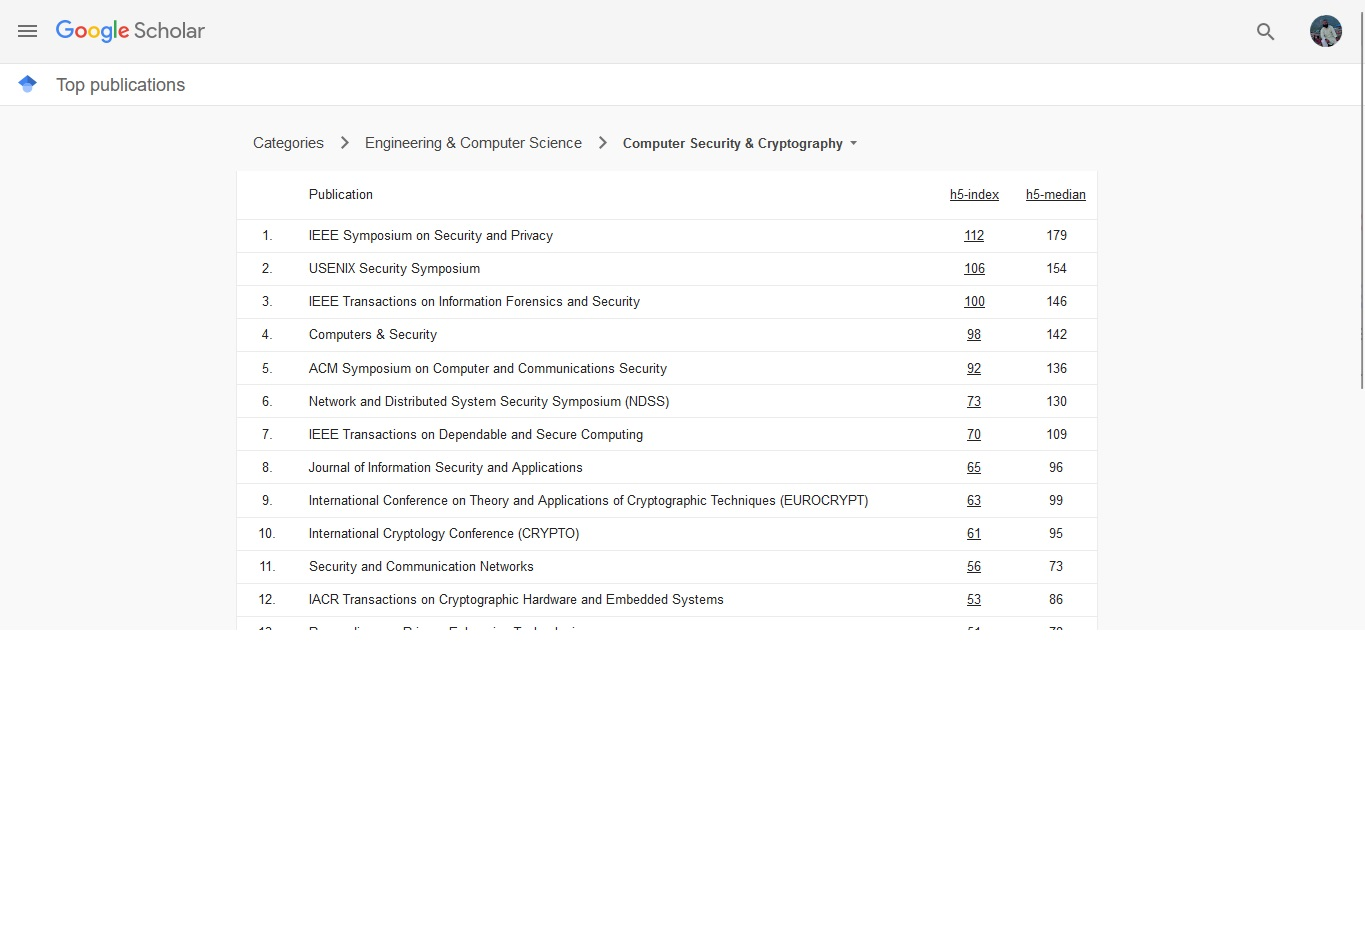
\includegraphics[width=\textwidth]{subcategory.jpg} 
    \caption{Best paper searching using metrics of google scholar }
    \label{fig:toc}
\end{figure}

\noindent\textbf{Paper 1:} \url{https://doi.org/10.32604/iasc.2022.019121} \\
Yousef S. Alshunaifi, Sudhir Mishra, and Mohammad Alshehri. (2022). \textit{Cyber-Attack Detection and Mitigation Using SVM for 5G Network}. Intelligent Automation \& Soft Computing, 31(1).\\

\noindent This paper addresses cybersecurity vulnerabilities in 4G and 5G networks, proposing an SVM-based intrusion detection system to enhance security. The research combines qualitative analysis through literature review and surveys with quantitative experimentation, demonstrating improved QoS metrics and effective cyber-attack detection and mitigation in 5G environments. I chose to scan this paper due to its closely relation with my research area and its  relevance in exploring machine learning techniques, specifically Support Vector Machine (SVM), for enhancing cybersecurity measures within next-generation networks, a critical area given the increasing threats in the telecommunications sector.\\

\noindent \textbf{Paper 2:} \url{https://doi.org/10.1109/MNET.011.2000088} \\
Yousef S. Alshunaifi, Sudhir Mishra, and Mohammad Alshehri. (2022). \textit{Cyber-Attack Detection and Mitigation Using SVM for 5G Network}. Intelligent Automation \& Soft Computing, 31(1).\\

\noindent This paper provides an overview of AI applications for security in future networks, covering topics like identity management, API security, anomaly detection, and root cause analysis. It offers concrete examples of how AI can be leveraged to address specific security challenges in next-generation mobile networks.I chose to scan this paper because it also close to my research area and  it directly addresses how AI can be used to enhance security in 5G and beyond networks, which seems most relevant to understanding AI's role in network security.\\

\noindent\textbf{Paper 3:} \url{https://doi.org/10.1109/TETC.2022.3147192} \\
T. Saha, N. Aaraj, and N. K. Jha. (2022). \textit{Machine learning assisted security analysis of 5G-network-connected systems}. IEEE Transactions on Emerging Topics in Computing, 10(4), 2006-2024.\\

\noindent This paper explores a machine learning-assisted framework to analyze the security vulnerabilities of 5G network core systems, focusing on attack graphs generated from SDN, NFV, and other 5G technologies. It identifies 119 novel possible exploits and discusses five new attack vectors compromising the 5G-AKA protocol, highlighting potential impacts on applications like WhatsApp.I chose to scan this paper because it directly relates to my research area, particularly focusing on anomaly detection and security issues in 5G networks, making it highly relevant to your thesis work on 5G/6G networks and security analysis.

\section{ Google Scholar Search}

Using Google Scholar, I identified 25 papers relevant to my research area, which focuses on cybersecurity in 5G/6G networks, machine learning for anonymous networking detection in cryptocurrency, and anomaly detection in fake base stations. Below are the details of the five papers I skimmed:\\

\noindent\textbf{Paper 1:} \textit{Scalise, P., Boeding, M., Hempel, M., Sharif, H., Delloiacovo, J., \& Reed, J. (2024). A Systematic Survey on 5G and 6G Security Considerations, Challenges, Trends, and Research Areas. Future Internet, 16(3), 67.} \\
\textbf{Time:} 1:45 minutes \\
This paper provides a comprehensive review of the security challenges in 5G and 6G networks, addressing emerging trends such as Zero Trust Architecture, blockchain, and post-quantum cryptography. It discusses vulnerabilities in key network components and proposes future security directions to enhance system integrity and privacy. \\

\noindent\textbf{Paper 2:} \textit{Nikula, M. M. (2024). Machine learning-based anomaly detection and root cause analysis in mobile networks.} \\
\textbf{Time:} 2:00 minutes \\
This thesis presents an unsupervised machine learning model using DBSCAN and LSTM Autoencoder to detect network anomalies and identify root causes in unlabelled 4G mobile network data. It highlights the model's effectiveness in enhancing network performance while emphasizing the challenges posed by unlabelled data. \\

\noindent\textbf{Paper 3:} \textit{Sakib, N., Wuthier, S., Zhang, K., Zhou, X., \& Chang, S. Y. (2024, May). From slow propagation to partition: Analyzing bitcoin over anonymous routing. In 2024 IEEE International Conference on Blockchain and Cryptocurrency (ICBC) (pp. 377-385). IEEE.} \\
\textbf{Time:} 1:30 minutes \\
The paper analyzes the performance of Bitcoin's peer-to-peer network when using anonymous routing technologies like Tor, I2P, and CJDNS. It finds that while anonymous routing helps protect user anonymity, it introduces delays and can lead to network partitioning, which negatively impacts Bitcoin's mining operations and consensus protocols. \\

\noindent\textbf{Paper 4:} \textit{Liwen, Z., Qamar, F., Liaqat, M., Hindia, M. N., \& Ariffin, K. A. Z. (2024). Towards Efficient 6G IoT Networks: A Perspective on Resource Optimization Strategies, Challenges, and Future Directions. IEEE Access.} \\
\textbf{Time:} 1:55 minutes \\
The paper presents resource optimization strategies to enhance the performance of 6G IoT networks. It emphasizes key performance indicators like latency, energy efficiency, spectrum efficiency, and bandwidth utilization while identifying future research directions and challenges related to optimizing resources in these networks. \\

\noindent\textbf{Paper 5:} \textit{Khazane, H., Ridouani, M., Salahdine, F., \& Kaabouch, N. (2024). A holistic review of machine learning adversarial attacks in IoT networks. Future Internet, 16(1), 32.} \\
\textbf{Time:} 1:40 minutes \\
The paper provides a comprehensive overview of adversarial attacks targeting machine learning-based security systems within IoT networks. It discusses various attack methods, including those on Intrusion Detection Systems (IDS), Malware Detection Systems (MDS), and Device Identification Systems (DIS), and proposes a taxonomy of attacks and defenses specific to the IoT environment. \\

\noindent For the remaining 20 papers, I group-cited them as they were relevant but did not require immediate in-depth reading.

\noindent \textbf{Group Citation:} 
% Include all entries from references.bib that have the keyword 'rest20'
\nocite{*}
\printbibliography[keyword={rest20}]

\section{ Browsing}

I selected the \textit{IEEE Transactions on Information Forensics and Security (TIFS)} journal for my browsing exercise. TIFS is one of the most prestigious journals in the field of cybersecurity, and it regularly publishes cutting-edge research on 5G/6G security, network anomaly detection, and machine learning for cybersecurity applications. I chose to browse two issues from the last two years, which included more than 45 papers in total.

\subsection{Screenshot of the Table of Contents}
\begin{figure}[ht]
    \centering
    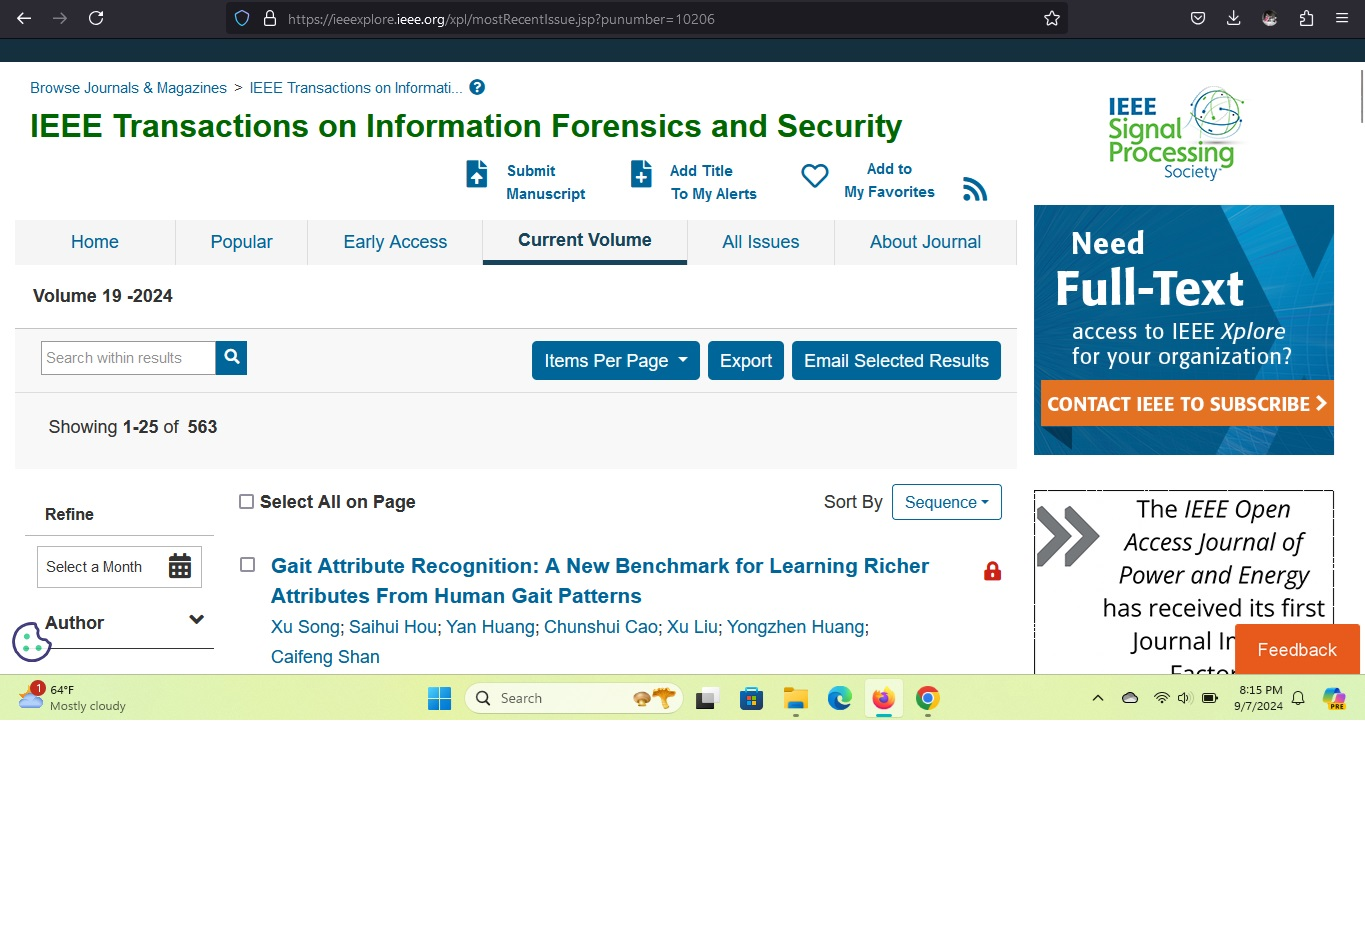
\includegraphics[width=\textwidth]{content.jpg} 
    \caption{Table of Contents from \textit{IEEE TIFS}, Volume 19, Issue 2024,2024}
    \label{fig:toc}
\end{figure}

I chose to browse TIFS because it covers a wide range of relevant topics for my research, including 5G/6G security, anomaly detection, and machine learning applications for cybersecurity which is shown in Figure 2. Through this exercise, I hoped to identify new advancements, methodologies, and practical challenges in the domain that could contribute to my ongoing research on anomaly detection in fake base stations and AI-based trend analysis in online networks. 

\subsection{Browse Timing Notes and Decisions}

For each of the 45 papers, I timed myself using a stopwatch, spending no more than 2 minutes per paper. Below is a summary of my timing, decisions, and BibTeX entries for these papers.
% Include all entries from references.bib that have the keyword '45'
\nocite{*}
\printbibliography[keyword={45}]

\subsection{Summary of Scanned Papers}

After browsing 45 papers, I decided to scan 8 of them in detail. Below is a brief summary of the most relevant papers:\\

\noindent\textbf{Paper 21:} The paper introduces a novel benchmark dataset and methodologies for identifying detailed human attributes based on their walking patterns. It aims to enhance gait-based recognition by extracting richer and more diverse attributes, improving the accuracy of identifying characteristics like gender, age, and movement style. This research has potential applications in security, healthcare, and biometrics.\\

\noindent\textbf{Paper 28:} The paper proposes a method to detect backdoor attacks in deep learning models by exploiting the non-transferability property of backdoor triggers. The approach aims to identify malicious behaviours embedded in models by distinguishing between clean and compromised inputs based on their inability to transfer across different models. This technique enhances model security by effectively detecting and mitigating hidden backdoor threats.\\

\noindent\textbf{Paper 32:} The paper  presents a game-theoretic approach to enhance the security of vehicle platoons against cyber-physical attacks. By modeling interactions between attackers and defenders as an adversarial game, the research explores strategies for vehicles to decide whether to act or not based on the perceived threat level. This framework aims to improve the resilience and safety of autonomous vehicle networks.\\

\noindent\textbf{Paper 35:} The paper introduces a secure approach to storing key-value data in cloud environments by using encryption and compression techniques. The proposed system ensures data confidentiality while defending against pattern-analysis attacks, which aim to exploit access patterns to uncover sensitive information. This method enhances the security and efficiency of cloud-based storage systems, balancing data protection with performance optimization.\\

\noindent\textbf{Paper 41:} The paper explores the use of frequency-mixing techniques to generate entropy for secure random number generation in hardware-based cybersecurity solutions. This approach leverages mixed frequencies to enhance the randomness and unpredictability of generated numbers, which is crucial for encryption and safe operations. The research focuses on portable hardware, offering a novel perspective on improving cybersecurity in embedded systems.\\

\noindent\textbf{Paper 45:} The paper introduces a method to enhance the accuracy of face and kinship verification systems by incorporating confidence calibration techniques. This approach aims to assess the reliability of verification results better, improving the system's performance in distinguishing between individuals and identifying family relationships. The proposed method enhances the robustness and precision of biometric systems by addressing the uncertainties inherent in face and kinship verification tasks.\\

\noindent\textbf{Paper 53:} The paper presents a novel approach to specific emitter identification under data constraints. The method leverages self-supervised learning to extract meaningful features from limited data and employs adversarial augmentation to generate synthetic samples, improving model robustness and performance. This approach addresses the challenge of scarce data by enhancing the ability to identify and classify emitters accurately with minimal training examples.\\

\noindent\textbf{Paper 63:}The paper explores methods for enabling accountable and precise modifications within blockchain systems. It introduces mechanisms for rewriting blockchain data while maintaining transparency and control over changes, addressing the challenges of immutability and accountability in decentralized ledgers. This approach allows for more flexible data management and correction while ensuring that modifications are traceable and controlled, enhancing the functionality and reliability of blockchain applications.

\subsection{Critical Reading of Best Papers}

After scanning, I chose to critically and creatively read the following papers, which align most closely with my research focus on cybersecurity:\\

\noindent\textbf{Paper 28:} The paper proposes a method to detect backdoor attacks in deep learning models by leveraging the non-transferability of backdoor triggers. This approach enhances model security by distinguishing between clean and compromised inputs, thereby identifying and mitigating hidden backdoor threats effectively.\\

\noindent\textbf{Paper 45:} The paper presents a method to improve face and kinship verification systems by using confidence calibration techniques to better assess the reliability of verification results. This approach enhances the system's accuracy in distinguishing individuals and identifying family relationships, addressing inherent uncertainties in biometric verification tasks.\\

\noindent  The browsing and scanning of papers from TIFS allowed me to gain valuable knowledge of the latest trends in cyber security and anomaly detection, which will be instrumental for my research.

%\bibliographystyle{IEEEtran}


\end{document}
